\setcellcolorrange{0}{60}{70}
\begin{table}[H]
\centering
\caption{Object base optimisation summary.}
\label{tab:object_technique_summary}
\footnotesize
\definecolor{rulegray}{gray}{0.88}
\begin{minipage}{0.35\linewidth}
\centering
\setlength{\tabcolsep}{4pt}
\begin{tabular}{l c c}
\toprule
\textbf{Technique} & \textbf{$\Delta$mAP} & \textbf{Lat.$\downarrow$} \\
\midrule
\textbf{Acceleration} & \autocolorcell{-0.3}{-0.3\%} & \autocolorcell{31.0}{31.0\%} \\

\arrayrulecolor{rulegray}\specialrule{0.35pt}{0pt}{0pt}\arrayrulecolor{black}

\multicolumn{3}{l}{\textbf{Input Scaling and Accel.}} \\
\hspace{1em}75\% & \autocolorcell{-3.1}{-3.1\%} & \autocolorcell{31.5}{31.5\%} \\
\hspace{1em}60\% & \autocolorcell{-9.1}{-9.1\%} & \autocolorcell{52.9}{52.9\%} \\
\hspace{1em}50\% & \autocolorcell{-15.4}{-15.4\%} & \autocolorcell{67.7}{67.7\%} \\

\arrayrulecolor{rulegray}\specialrule{0.35pt}{0pt}{0pt}\arrayrulecolor{black}

\multicolumn{3}{l}{\textbf{Quantisation}} \\
\hspace{1em}FP16 & \autocolorcell{-1.6}{-1.6\%} & \autocolorcell{42.8}{42.8\%} \\
\hspace{1em}INT8 & \autocolorcell{-9.9}{-9.9\%} & \autocolorcell{52.6}{52.6\%} \\

\arrayrulecolor{rulegray}\specialrule{0.35pt}{0pt}{0pt}\arrayrulecolor{black}

\multicolumn{3}{l}{\textbf{Pruning}} \\
\hspace{1em}90\% pruning & \autocolorcell{-1.6}{-1.6\%} & \autocolorcell{2.3}{2.3\%} \\
\hspace{1em}80\% pruning & \autocolorcell{-2.4}{-2.4\%} & \autocolorcell{2.8}{2.8\%} \\
\hspace{1em}70\% pruning & \autocolorcell{-4.6}{-4.6\%} & \autocolorcell{13.4}{13.4\%} \\

\arrayrulecolor{rulegray}\specialrule{0.35pt}{0pt}{0pt}\arrayrulecolor{black}

\multicolumn{3}{l}{\textbf{Distillation}} \\
\hspace{1em}Small jump & \autocolorcell{-1.1}{-1.1\%} & \autocolorcell{-13.3}{-13.3\%} \\
\hspace{1em}Medium jump & \autocolorcell{-0.7}{-0.7\%} & \autocolorcell{-10.7}{-10.7\%} \\
\hspace{1em}Large jump & \autocolorcell{-2.1}{-2.1\%} & \autocolorcell{-8.7}{-8.7\%} \\
\bottomrule
\end{tabular}
\end{minipage}
\hfill
\begin{minipage}{0.64\linewidth}
\centering
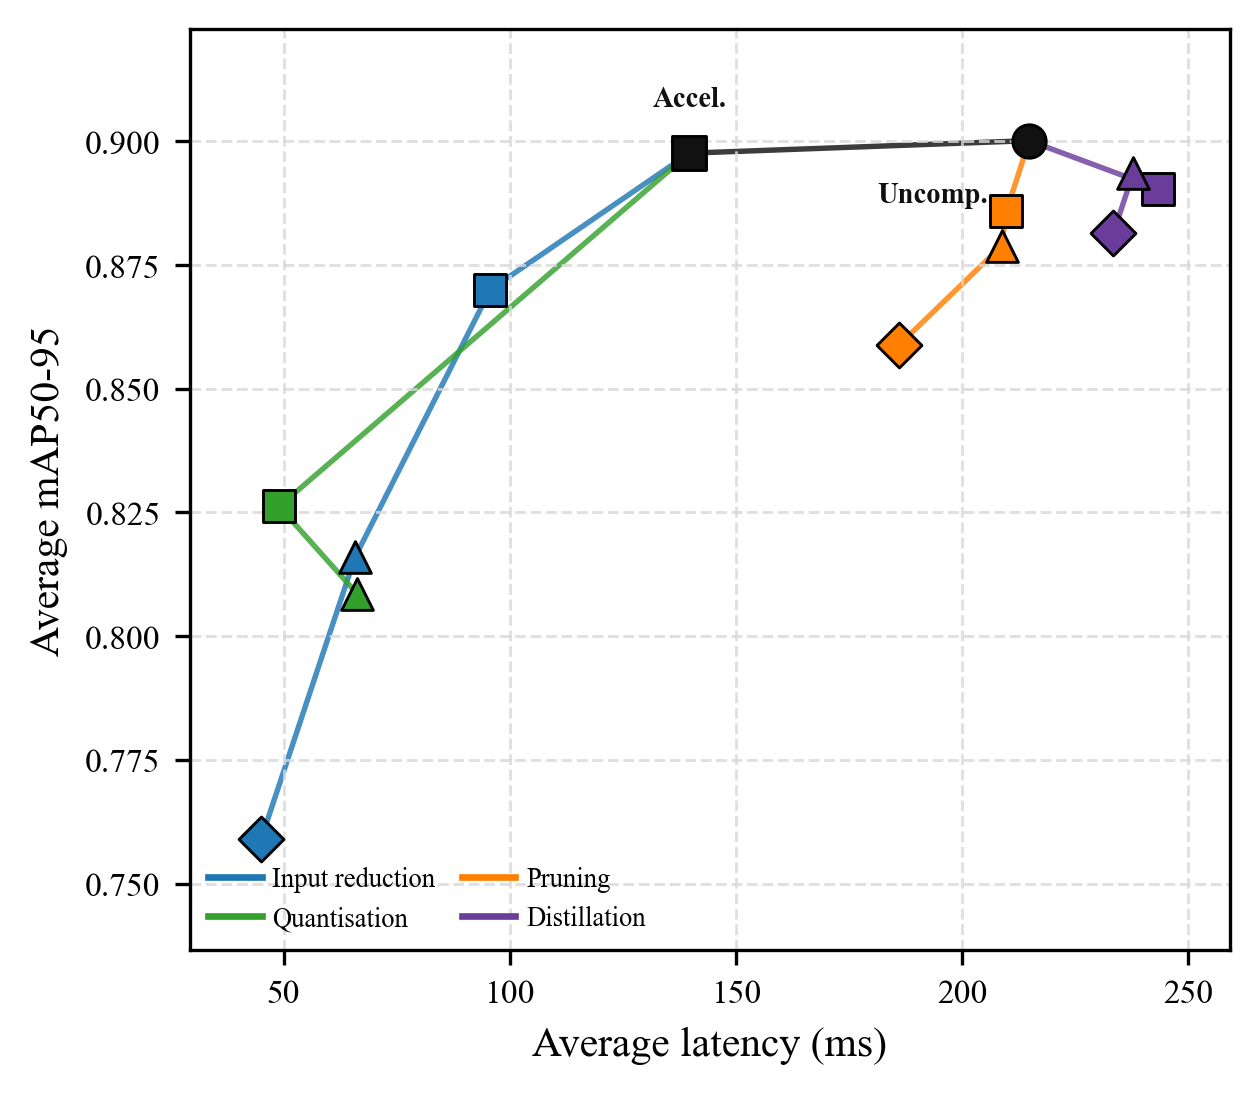
\includegraphics[width=\linewidth]{../Figures/produced_images/object_technique_summary_tradeoff.png}
\end{minipage}

\par
\vspace{3pt}
\noindent\parbox{\linewidth}{\footnotesize \textit{Note:} Distill Jump sizes defined by gap to teacher: small=1 size up, medium=2 sizes, large=3+ sizes up.}
\end{table}
